%\documentclass[journal=jacsat,manuscript=article]{achemso}
\documentclass{article}

\usepackage{amssymb}

\usepackage{graphicx}

%opening
\title{Avogadro: A Framework and Cross Platform GUI for Building Molecular Structures and the Analysis of Output}

%% Uncomment these when using the acs document style

%\author{Marcus D. Hanwell}
%\author{Geoffrey R. Hutchison}
%\email{geoffh@pitt.edu}
%\affiliation[Pitt]{Department of Chemistry, University of Pittsburgh, PA, USA.}

%\author{Donald E. Curtis}
%\affiliation[Iowa]{Department of Computer Science, University of Iowa, USA.}
%\author{Tim Vandermeersch}
%\affiliation[Unknown]{Department of , University of Unknown.}

\begin{document}

\maketitle

\begin{abstract}

Avogadro is a free, cross-platform, open source, OpenGL based graphical user
interface and library for building molecular structures, formatting input files
and analyzing output files from computational chemistry codes. The work
presented here details the Avogadro library, which provides a framework,
application programming interface, and three-dimensional visualization
capabilities that have direct applications in research and education in the
fields of chemistry, physics, materials science and biology. The Avogadro
application provides a rich graphical interface using dynamically loaded plugins.
The application can be extended by implementing a plug-in module in C++ or Python in
order to explore different visualization techniques, build/manipulate molecular
structures, and interact with other programs.
We describe some example extensions, one which uses a genetic algorithm to find
stable crystal structures, and one which interfaces with the PackMol program to
create packed, solvated structures for molecular dynamics simulations.

\end{abstract}

\section{Introduction}

Many areas such as chemistry, materials science, physics and biology need efficient computer programs to both build and visualize molecular structures. The field of molecular graphics is dominated by viewers with little or no editing capabilities, such as RasMol~\cite{RasMol}, JMol~\cite{JMol}, PyMOL~\cite{PyMOL}, VMD~\cite{VMD}, QuteMol~\cite{QuteMol}, and BALLView~\cite{BALLView} among many others. The aforementioned viewers are all freely available, and most of them are available under open source licenses and work on the most common operating systems (GNU/Linux, Apple Mac OS X, BSD and Microsoft Windows).

The choice of software capable of building chemical structures is far smaller. There are existing commercial packages, such as Spartan, CAChe, GaussView, Materials Studio~\cite{Accelrys} and CrystalMaker~\cite{CrystalMaker}, that are well polished and capable of constructing many different types of molecular structures. They are however not available for all operating systems (most of them only have programs for Microsoft Windows), are not easily extensible or released under an open source license. Licensing costs can be prohibitive, as can the changing direction of companies which can lead to a loss of significant research investment in a single commercial product.

The selection of free, open source, cross platform molecular builders was quite limited when the Avogadro project was founded in late 2006. Ghemical~\cite{Ghemical} was one of the only projects satisfying these needs at the time. Two of the authors (Hutchison and Curtis) contributed to Ghemical previously, but had found that it was not easily extensible. This led them to found a new project in order to address the issues they had observed in Ghemical and other packages. The Molden~\cite{Molden} application was also available, able to build up small molecules and analyze output from several quantum codes. It suffers from a restrictive license and also uses an antiquated graphical toolkit.

Following a case study of the available applications capable of building molecular structures broad design goals were outlined. One of the main issues with both commercial and open source applications is a lack of extensibility, many of the applications also only work on one or two operating systems. An open and extensible framework is needed in order to be able to perform innovative research. The creation of a framework that implements many of the necessary foundations for a molecular builder and visualizer would facilitate more effective research in this area in the future.

At the time of writing it is apparent that other researchers have perceived similar needs. Several new applications are available today that focus on both building and visualizing molecular structure. These include CCP1GUI~\cite{CCP1GUI}, Gabedit~\cite{Gabedit} along with some highly specific editors such as MacMolPlt~\cite{MacMolPlt}. Whilst offering many interesting and useful features, these projects suffer from the same kind of issues centering around effective reuse of existing code, well commented and documented code and easy extension to specialized areas.

The Avogadro project has endeavored to make a free, open source framework for both building and visualizing molecular structures. Much of the initial focus has been placed on preparing input and analyzing output from quantum calculations. Other applications such as preparing input for MD simulations and visualizing periodic structures will also be presented, demonstrating the flexibility of the Avogadro framework.

Avogadro has close ties to several other free, cross platform, open source projects in order to reuse as much code as is practical. These projects include Nokia Qt to provide a free, cross platform graphical toolkit, Open Babel~\cite{OpenBabel} for chemical file input/output, geometry optimization and other chemical perception, Eigen~\cite{Eigen} for matrix and vector mathematics, OpenGL/GLSL for real time three dimensional rendering and POV-Ray for ray-traced rendering.

Avogadro also uses quantum codes such as GAMESS-US, Q-Chem, Gaussian and MOPAC to perform ab-initio and semi-empirical calculations. Support for more calculation backends is planned and we are working with Q-Chem on an advanced input file generator. As with most open source projects, the directions the project has taken were influenced largely by the research areas and interests of the principal contributors.

\section{The Graphical User Interface}

%The first thing most people will see is the main Avogadro application window. Binary installers are provided under the GPL license for Apple Mac OS X and Microsoft Windows, along with packages for all of the major Linux distributions. This means that Avogadro can be installed quite easily on most operating systems. Easy to follow instructions on how to compile the latest source code are also provided on the main Avogadro web site for the more adventurous, or those using an operating system that is not yet supported.

%The Qt toolkit from Nokia gives Avogadro a native look and feel on the three supported operating systems---Linux, Mac OS X and Windows. The basic functionality expected in a molecular builder and viewer has been implemented, along with several less common features. The vast majority of this functionality has been written using the API made available to plug-in writers, and is loaded at runtime. It is very easy for new users to install Avogadro and build their first molecules within minutes. Thanks to the Open Babel library Avogadro supports a large portion of the chemical file formats that are in common use.

The first thing most people will see is the main Avogadro application window.
The basic functionality expected in a molecular builder and viewer has been
implemented, along with several less common features. The vast majority of this
functionality has been written using the API made available to plugin writers,
and is loaded at runtime. It is very easy for new users to install Avogadro and
build their first molecules within minutes. Thanks to the Open Babel library
Avogadro supports a large portion of the chemical file formats that are in
common use.
% TODO Update the figure here
\begin{figure}
  \begin{center}
    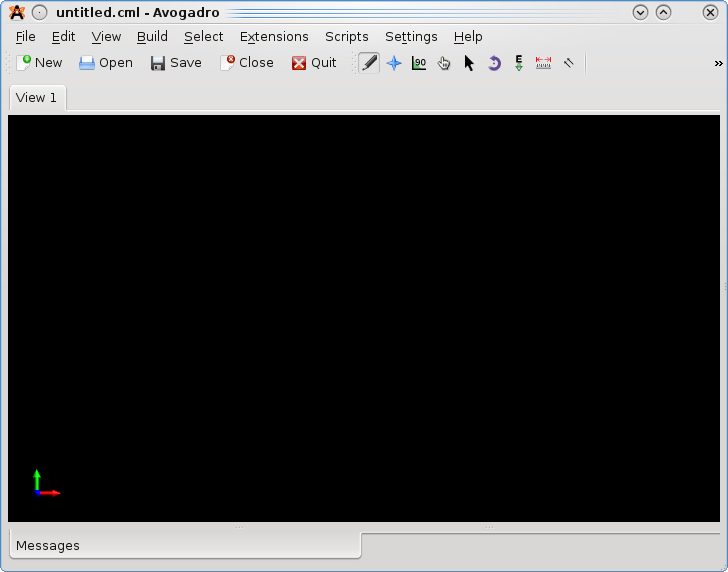
\includegraphics[width=0.8\textwidth]{images/avogadro-0-9-8}
  \end{center}
  \caption{The Avogadro graphical user interface when first opened.}
  \label{f:avogadrogui}
\end{figure}


\subsection{Building a Molecule: Atom by Atom}

After opening Avogadro a window such as that shown in figure~\ref{f:avogadrogui} is presented. From there simply left clicking on the black part of the display allows the user to draw a carbon atom. If the user pushes the left mouse button down and drags a bonded carbon atom would be drawn between the start point and the final position where the mouse was released.

A large amount of effort has been expended to create an intuitive tool for drawing small molecules. Common elements can be selected from a drop down list, or a periodic table can be displayed to select less common elements. Clicking on an existing atom changes its type, dragging reverts the original atom and draws the new atom bonded to the original. If the bonds are left-clicked then the bond order cycles between single, double and triple.

Right clicking on atoms or bonds deletes them. If the ``Adjust Hydrogens'' box is checked the number of hydrogens bonded to each atom is automatically adjusted to satisfy valency. This can also be done at the end of an editing session by using the add hydrogens extension in the build menu. Keyboard shortcuts are also available to change the active element (by typing the one or two letter symbol), or bond order (by entering the numeric bond order).

In addition to the draw tool there are two tools for adjusting the position of atoms in existing molecules. The atom centric manipulate tool can be used to move an atom or a group of selected atoms. The bond centric manipulate tool can be used to select a bond and then adjust all atoms positions relative to the selected bond in various ways. These three tools allow for a great deal of flexibility in building small molecules interactively on screen.

Once the molecular structure is complete the forcefield extension can be used to perform a geometry optimization. By clicking on ``Extensions'' and ``Optimize Geometry'' a fast geometry optimization is performed on the molecule. The forcefield and calculation parameters can be adjusted, but the defaults are adequate for most molecules. This workflow is typical when building up a small molecular structures for use as input to quantum calculations, or publication quality figures.

An alternative is to combine the ``Auto Optimization'' tool with the drawing tool. This presents a unique way of sculpting the molecule while the geometry is constantly minimized in the background. The geometry optimization is animated, and the effect of changing bond orders, adding new groups or removing groups can be observed interactively.

Several dialogs are provided to provide information on molecule properties, and to precisely change parameters, such as the cartesian coordinates of the atoms in the molecule.

\subsection{Building a Molecule: From Fragments} %Geoff?

\begin{figure}
	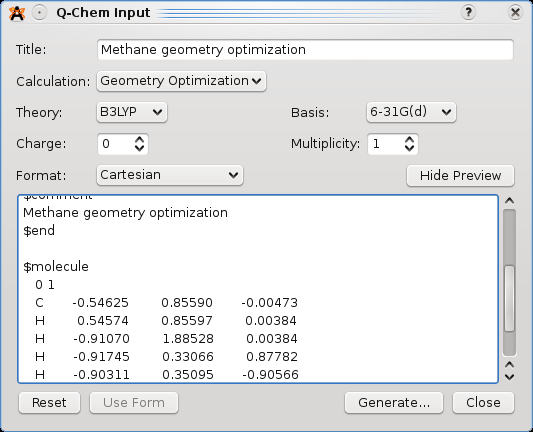
\includegraphics[width=0.44\textwidth]{images/avogadro-q-chem}
	\hspace{0.1cm}
	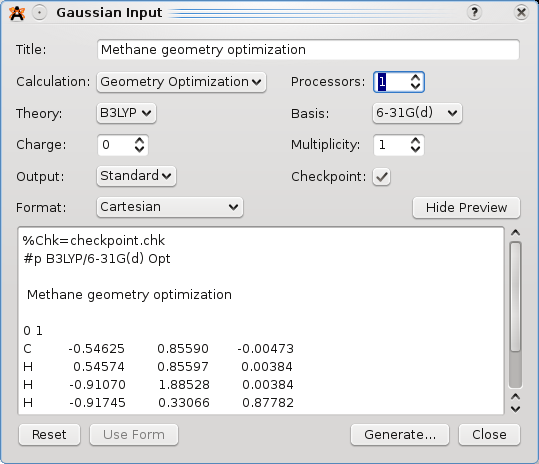
\includegraphics[width=0.44\textwidth]{images/avogadro-gaussian}
	\caption{Dialog for generating input for Q-Chem (left) and Gaussian (right).}
	\label{f:quantumdialogs}
\end{figure}

\subsection{Preparing Input for Quantum Codes}

Several extensions were developed for Avogadro that assist the user in preparing input files for popular quantum codes such as GAMESS-US, Gaussian, Q-Chem and MOPAC. The graphical dialogs present the features required to run basic quantum calculations, some examples are shown in figure~\ref{f:quantumdialogs}.

The preview of the input file at the bottom of each dialog is updated as options are changed. This approach helps new users of quantum codes to learn the syntax of input files for different codes, and to quickly generate useful input files as they learn. The input can be edited in the dialog, before the file is saved and submitted to the quantum code. The MOPAC extension can also run the  MOPAC program directly if it is available on the user's computer, Avogadro can also load the output file once the calculation is complete.

\subsection{Alignment and Measurements}

One of the specialized tools included in the standard Avogadro distribution is the alignment tool. This mouse tool facilitates the alignment of a molecular structure with the coordinate origin if one atom is selected, and along the specified axis if two atoms are selected. The alignment tool can be combined with the measure, select and manipulate tools in order to create inputs for quantum codes where the position and orientation of the molecule is important. One example of this is calculations where an external electric field is applied to the molecule. In these types of calculations the alignment of the molecule can have a large effect.

More complex alignment tools for specific tasks couuld be created. The alignment tool was created in just a few hours for a specific research project performing calculation on the piezoelectric effect in single molecules. This is a prime example where extensibility was very important in order to be able to perform research using a graphical computational chemistry tool. It would not have been worth the investment to create a new application just to align molecular structures to an axis, but creating a plugin for an extensible project was not unreasonable.


\section{Visualization}

The Avogadro application uses OpenGL to render molecular representations to the screen interactively. This has the advantage of being a good cross platform API to render three dimensional images using hardware accelerated graphics. OpenGL 1.1 and below is used in most of the rendering code, and so Avogadro can be used even on very modest/old computer systems. It is capable of taking advantage of some of the newer features available in OpenGL 2.0, but this has been kept as an optional extra feature when working on novel visualizations of molecular structure.

\subsection{Standard Representations}

\begin{figure}
	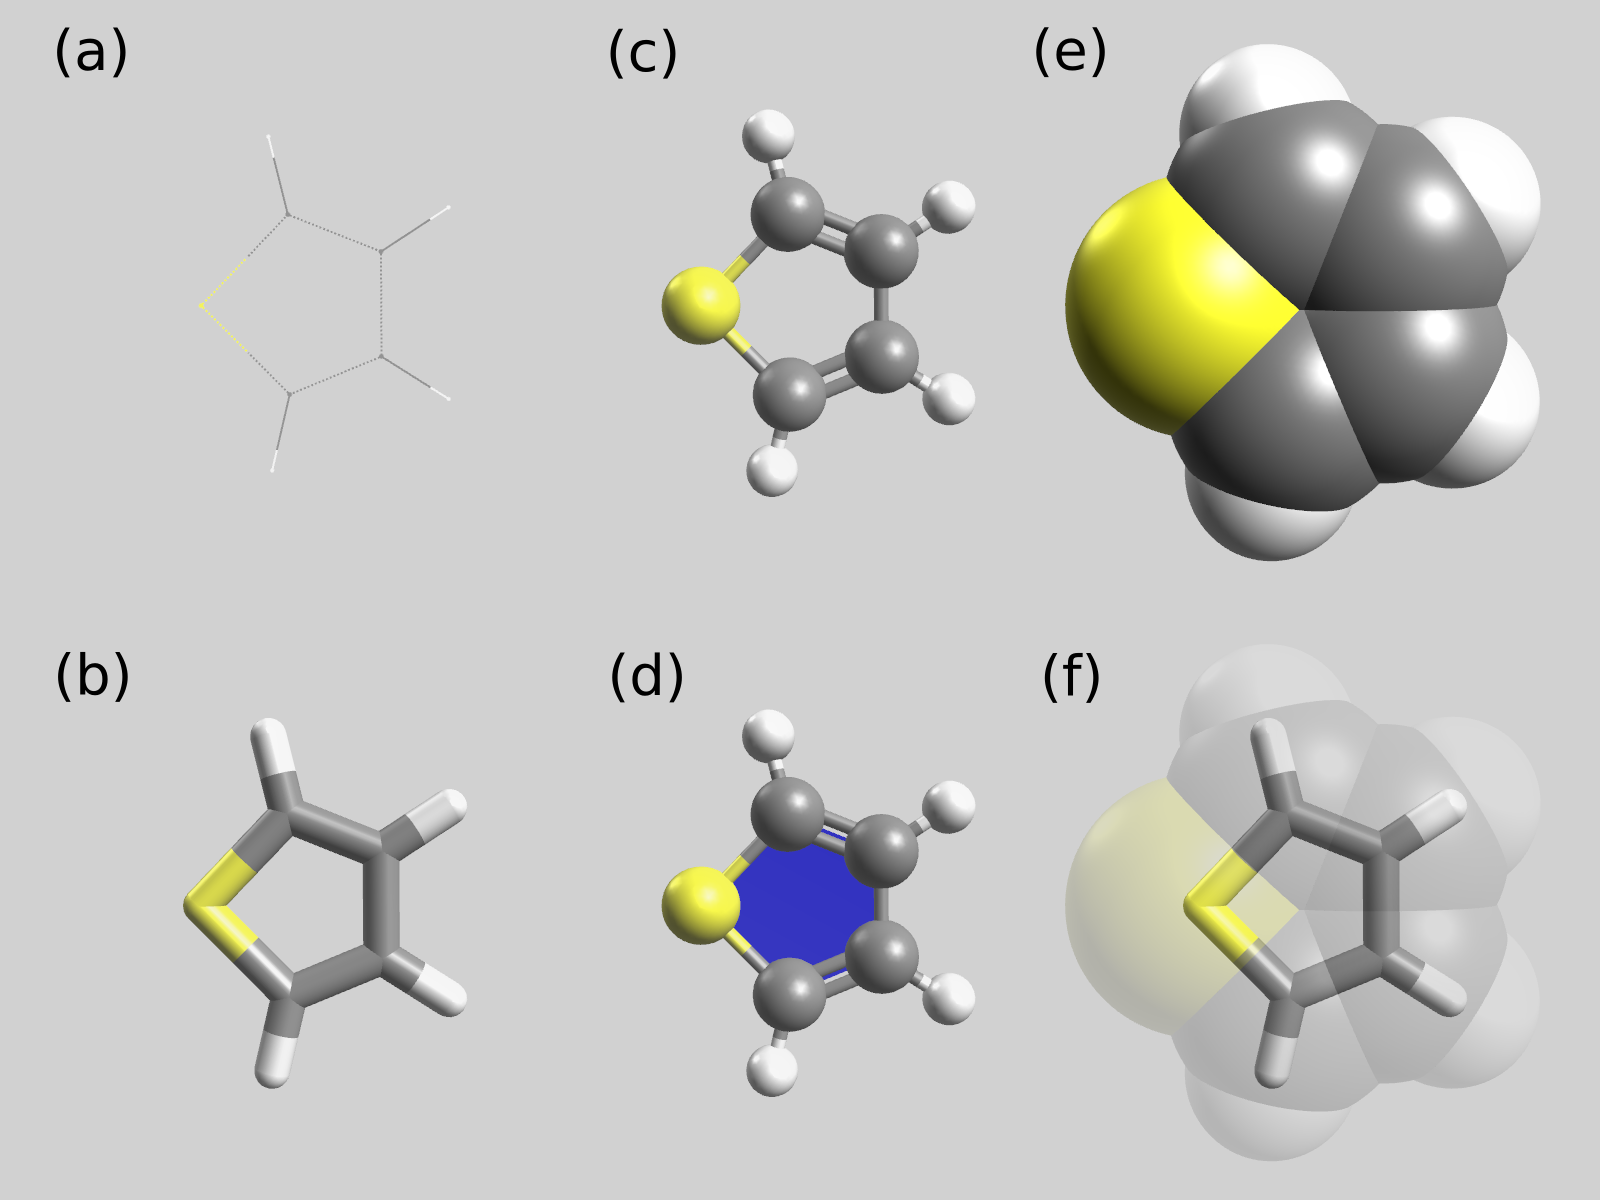
\includegraphics[width=0.95\textwidth]{images/standardRepsLabel}
	\caption{Several molecular representations of thiophene, (a) wireframe, (b) stick/liquorice, (c) ball and stick, (d) ball and stick with ring, (e) Van der Waal's/CPK and (f) transparent Van der Waal's with stick.}
	\label{f:standardReps}
\end{figure}

In chemistry there are several standard representations of molecular structre, originally based upon those possible with physical models. The Avogadro application implements each of these representations shown in figure~\ref{f:standardReps} as a plugin. These range from the simple wireframe representation, stick/liquorice, ball and stick and Van der Waal's.

It is also possible to combine several representations, such as ball and stick with ring rendering, figure~\ref{f:standardReps} (d), and a semi-transparent Van der Waal's space-filling representation with a stick representation to eludicate molecular backbone, figure~\ref{f:standardReps} (f).

\subsection{Electronic Structure}

Avogadro can read Gaussian cube files, in addition it can also read the basis set and relevant information output by Gaussian, Q-Chem, Molpro and MOPAC. The volumetric data can be calculated and isosurfaces computed from that volumetric data. There are display types that can display these isosurfaces in Avogadro interactively.

\subsection{Secondary Biological Structure} % This would likely be a great one for Tim to add some detail to.

\subsection{GLSL, Novel Visualization}



\subsection{Ray Tracing}

Description and examples of ray traced images.

\section{Software Architecture}

One area that seems to suffer in many code bases in chemistry is software architecture. This can lead to less maintainable code, poor code reuse and a much higher barrier to entry. Problems were identified in other projects with a view to minimizing their impact when developing Avogadro. Modern software design processes were used in the initial planning stages of Avogadro, along with the choice of modern programming languages and libraries.

Based on the previous experience of the authors, and a review of available programs at the time, several fundamental choices were made. The C++ programming language was chosen, with Qt as the cross platform graphical toolkit, OpenGL for 3D rendering, CMake as the build system and Open Babel as the chemical library. Using this combination of languages and libraries allowed for the project to be licensed under the GNU GPLv2 license and made (and kept) openly available to all.

The choice of license is an interesting one, and is hotly debated in many industries. The choice of the GPLv2 was necessitated because of the use of the Qt and Open Babel libraries. Qt has since been released under the much more permissive LGPL license. Packages such as PyMol use the more permissive BSD license, selling commercial versions in addition to the open source version (that has some capabilities missing that are present in the commercial version). The GPLv2 license is a good choice in order to ensure that the code base remains free and open, philosophically blocking the commercialization of the code at no cost to the company. This allows for open collaboration but precludes some avenues for funding further development.

The core of Avogadro is written in portable C++ code with platform specific differences abstracted away by Qt, OpenGL and Open Babel. The CMake build system makes the build process relatively simple on all supported platforms. Avogadro has been successfully built and tested on x86 and x86\_64 versions of Linux, PPC and x86 version of Apple Mac OS X and x86 Microsoft Windows. By leveraging the power of existing libraries the time required to develop new features has been significantly reduced.

Avogadro has a well defined set of interfaces and programming interfaces. Almost all functionality is implemented in self contained plugins that are loaded at runtime. The majority of these plugins are written in C++ but the Avogadro API has also been exposed to the Python scripting language. This allows for a great deal of choice in how plugins are implemented. In both cases each plugin is a self contained class that implements a set of functions that are part of the Avogadro API, allowing for a wide variety of features to be implemented in a very modular way.

The Avogadro framework uses the model, view, controller paradigm. The model being the core data classes such as Molecule, Atom and Bond, the view being the engine plugins and the controllers being the tools (interactive mouse) and extensions (non-interactive, form based/menu based). Each plugin has full access to the core data model.

\subsection{Plug-in Interface}

Description of the runtime plugin interface, along with some examples of the API for a typical plugin in C++ and Python.

\subsection{Display Types}

Display types are one type of plugin, referred to as engines internally. Their primar focus is with rendering graphics to the screen. As is the case with most molecular graphics a large portion of the geometric primitives are spheres and cylinders. These are typically used to represent atoms and bonds.

Some of the engines also convey some information about the underlying data the geometric primitives represent, in order to allow for the molecule to be edited. Engines are performance critical as the render functions are called each time a frame is requested for display. It is very important for the engines

\subsection{Tools}

\subsection{Extensions}

\subsection{Colors} % Geoff

\section{Python Interface} % Tim

Description of the Python bindings, PyQt, plugins as Python classes.

\section{Quantum Calculations}

Description of the quantum calculation code already implemented. Slater and Gaussian types, output file parsing, parallel calculation code and details of data layout.

\section{Avogadro Library in Use}

The Avogadro library used in Kalzium, may be Kompound if there is more to show. QUI as an external user, not yet well integrated.7

\section{Conclusions}

\bibliographystyle{unsrt}
\bibliography{AvogadroPaper}

\end{document}
